% \todo[inline]{MJ: In light of the methodology vs. data sources separation we agreed during the 26/03 meeting, I assume
% the following will have been discussed in the preceding methodology section:
% 1) We use a list of top ranked domain names to investigate how PCS behave
% across a diverse range of domains \ldots ({\bf without} already specifying
% Tranco); and 2) we identify content categories such as porn and gambling in the
% input domains using domain classification data ({\bf without} already
% specifying Cisco Umbrella Investigate API).}

In the following sections we provide details on our list of input domains and the classification data.

\subsection{List of Input Domains}
\label{sec:dataset:input_domains}

We use the Tranco Top 1 Million (downloaded on 19-02-2025, root domains) for our list of diverse input domains.
Tranco\footnote{\url{https://tranco-list.eu/}} is a research-oriented ranking
of the most-visited websites and includes domains spanning a variety of content
categories such as social media, news and search engines.
The list aggregates multiple other top lists, including Cloudflare Radar, the
Cisco Umbrella Popularity List, the Majestic Million, and the Crome User
Experience Report (CrUX). As Tranco aggregates these lists it addresses some of
their shortcomings, which include instability, inter-list disagreement, and
susceptibility to rank manipulation.
We use the standard version of the list with apex domains.
%\todo[inline]{MJ: to add: date(s)/snapshot(s) of Tranco list used. Readers may want to know.}

\subsection{Input Data for Domain Classification}
\label{sec:dataset:classification_data}

% \todo[inline]{MJ: from AA I understand that the Cisco API offers subdomain
% categorization. This raises a question: does PCS behavior change with subdomain granularity? If the
% answer is maybe, then, considering that you worked with Tranco root domains (while a subdomains list is also available), we need to
% probably describe as limitation that the findings are scoped to root-level domain behavior.}
% \todo[inline]{Anna: I added root domains to the Tranco paragraph, and add a few lines about this in the limitations}
%\todo[inline]{MJ: Let's avoid the term ``reclassification'' but rather use ``collate``, ``group`` and ``consolidate``}

We use the Cisco Umbrella Investigate API for domain name classification.
The \emph{domain status and categorization} data\footnote{\url{https://umbrella.cisco.com/products/umbrella-investigate}}
offers a detailed set of categories. To make these data more manageable and
relevant for evaluating parental controls, we developed a heuristic to
consolidate the categories into a smaller and simplified set. This
is guided by three key principles:

\begin{enumerate}
    \item We analyze the co-occurrence of categories across all input domains
        to identify cases where multiple categories are frequently assigned to
        the same domain (an example will follow in~\cref{sec:dataset:tranco_categories}).
        Such categories are candidates to be collated into a simpler category;
    \item We then collate similar and overlapping categories that provide additional
        granularity but no meaningful distinction in terms of web content
        filtering. For example, we merge \emph{Radio}, \emph{Music}, and
        \emph{Entertainment} into the simpler \emph{Entertainment};
    \item We consider categories through the specific lens of parental
        control system evaluation, and infer if a category should
        typically be blocked for children. For example, we expect the simpler \emph{Adult Content} category, which 
        collates Cisco categories such as \emph{Pornography} and \emph{Dating}, to not be meant for children.
\end{enumerate}

This results in a simplified, content-oriented classification that facilitates
the measurement of blocking behavior across different parental control
solutions.  The consolidated categories serve as the basis for our
exploration of which types of content are blocked by each parental control system.

\begin{figure}[!tb]
    \centering
    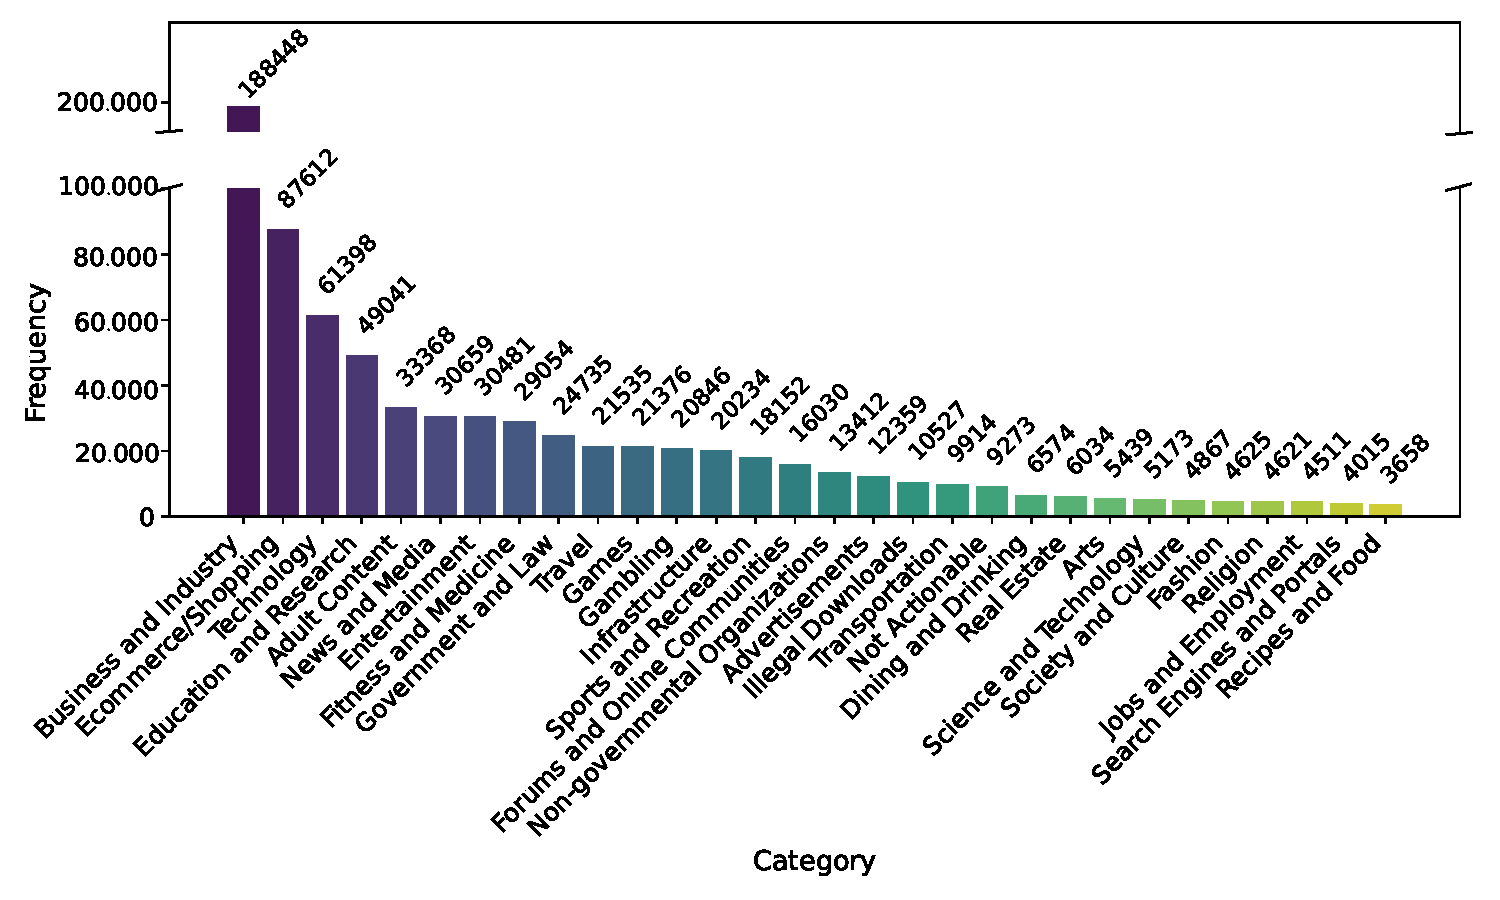
\includegraphics[width=1\columnwidth]{Images/top_30_categories.pdf}
    \caption{Tranco Lisy Top 30 Content Categories by Frequency.}
    \label{fig:top30categories}
\end{figure}

\subsection{Content Distribution Across Input Domains}
\label{sec:dataset:tranco_categories}

We mapped the Tranco list to categories to understand the distribution of content.
We were able to map 779,591 domains using the Cisco data. For the other 220,409 domains the Cisco data
does not offer a category.
%\todo{AA(?): we need to decide how to show these domains}
Figure\ref{fig:top30categories} shows the most prevalent categories among the Tranco domains.

Further analysis revealed that uncategorized domains appear more frequently
toward the long tail of the list. Only 8K domains missing a category are among
the Top 100K of the Tranco list.  We can only speculate as to the reasons for
this difference, but the position of domains in the list suggests that
categorization services may be more effective for high-traffic domains.
%, and may struggle with newly registered or obscure domains.

% \todo[inline]{AA: I think we need to make some analysis before making this claim; MJ: instead of analysis, is this something Cisco (or related work in this space) could confirm/support?}
% \todo[inline]{ML: This is not something that is based on anything i found in the literature, its pure speculation on my side simply based on the increasing number of unknown domains in the latter part of the list, if CISCO can confirm it ok, otherwise if the claim is too strong (even in this form) we will have to change it}
% \todo[inline]{Ale: The question is how excluding the non-ranked domains would impact the results? If we have restricted the blocking analysis to domains that have a cathegory, we can simply remove such a speculation and say something like "we concentrate on domains with a cathegory and we verified that domains without any cathegory are tipycally low ranking ones".}
% \todo[inline]{Anna: Answering Alessio: no, we did not restrict the analysis to having a category. I decided to tame down the claim by removing the part about struggling. The part about being more effective is speculative, but we are clear about it}

We next analyzed the extent to which domains were assigned multiple categories.
The vast majority of domains (95\%) mapped to a single class, with fewer than
4\% assigned two classes, and less than 0.5\% assigned three or more.
We conducted an analysis of category co-occurrences, which revealed that
several classes appeared together so frequently that they effectively
functioned as a single category, validating our intuition to collate and simplify categories.
For example, the \emph{Shopping} category co-occurred with
\emph{Ecommerce/Shopping} in 86,7K cases, while the prior appeared without the
latter fewer than 2K times.

By collating Cisco categories into simpler ones, we reduced the number of domains still assigned
multiple categories by several orders of magnitude, from hundreds
of thousands to a few thousand at most.
Of the consolidated categories, we consider \emph{Adult Content},
\emph{Gambling}, \emph{Hate/Discrimination} and \emph{Terrorism} to likely be
candidates for blocking by parental control systems. In the remaining of this paper, we will use those categories as reference for comparing the blocking capabilities of different solutions.
%\todo[inline]{AA: but we query all the domains, ?!}
In Figure~\ref{fig:blockedcategories} we show the cumulative distribution of
domains under these four categories in order of rank.
As shown, the number of domains belonging
to \emph{Hate/Discrimination} and \emph{Terrorism} is extremely low, while
\emph{Adult Content} and \emph{Gambling} are much more prevalent. In general, we observer that domains in these categories are quite evenly spread throughout the entire Tranco list.

\begin{figure}[!t]
    \centering
    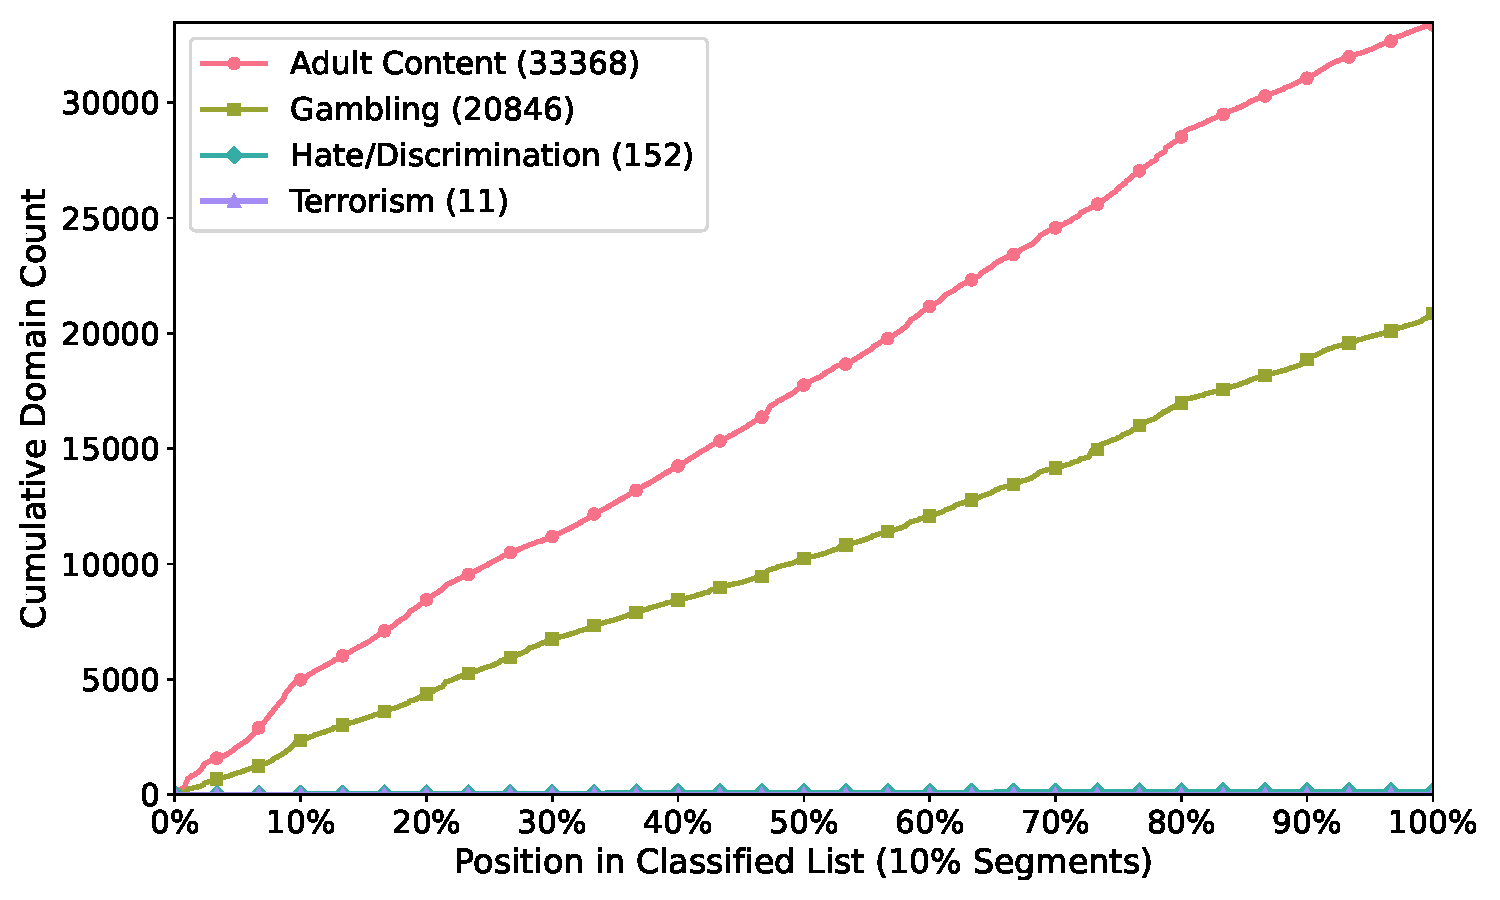
\includegraphics[width=0.95\columnwidth]{Images/cumulative_blocked_categories.pdf}
    \caption{Distribuion of Domains in Sensitive Categories.}
    \label{fig:blockedcategories}
\end{figure}

%\todo[inline]{AA: Increase the font size of the text in the figures.}
%\todo[inline]{AA(?): Update the numbers}
% \todo[inline]{Ale: I do not get the reason for this figure: why only these cathegorie? Do they sum up to the total number of domains considered? Using log scale for y axis would improve the visibility of the hate and terrorism. In general, a more detailed explanation is needed if we leave it.}
% \todo[inline]{Anna: I now explicitly added that we will use those categories as reference to measure the blocking capabilities. At least it makes sense to show something more about them in this way. I also added that they are evenly spread in the dataset. I know it is not very detailed}
